%%%%%%%%%%%%%%%%%%%%%%% file template.tex %%%%%%%%%%%%%%%%%%%%%%%%%
%
% This is a general template file for the LaTeX package SVJour3
% for Springer journals.          Springer Heidelberg 2010/09/16
%
% Copy it to a new file with a new name and use it as the basis
% for your article. Delete % signs as needed.
%
% This template includes a few options for different layouts and
% content for various journals. Please consult a previous issue of
% your journal as needed.
%
%%%%%%%%%%%%%%%%%%%%%%%%%%%%%%%%%%%%%%%%%%%%%%%%%%%%%%%%%%%%%%%%%%%
%
% First comes an example EPS file -- just ignore it and
% proceed on the \documentclass line
% your LaTeX will extract the file if required
\begin{filecontents*}{Heatmap.eps}
%!PS-Adobe-3.0 EPSF-3.0
%%BoundingBox: 19 19 221 221
%%CreationDate: Mon Sep 29 1997
%%Creator: programmed by hand (JK)
%%EndComments
gsave
newpath
  20 20 moveto
  20 220 lineto
  220 220 lineto
  220 20 lineto
closepath
2 setlinewidth
gsave
  .4 setgray fill
grestore
stroke
grestore
\end{filecontents*}
%
\RequirePackage{fix-cm}
%
%\documentclass{svjour3}                     % onecolumn (standard format)
%\documentclass[smallcondensed]{svjour3}     % onecolumn (ditto)
%\documentclass[smallextended]{svjour3}       % onecolumn (second format)
\documentclass[twocolumn,natbib]{svjour3}          % twocolumn
%
\smartqed  % flush right qed marks, e.g. at end of proof
%
\usepackage{graphicx}
\usepackage{amssymb}
\usepackage{amsmath}
\usepackage{algorithm}
\usepackage{url}
%\usepackage[linkcolor=blue,citecolor=blue]{hyperref}
%
% \usepackage{mathptmx}      % use Times fonts if available on your TeX system
%
% insert here the call for the packages your document requires
%\usepackage{latexsym}
% etc.
%
% please place your own definitions here and don't use \def but
\newcommand{\T}{{ \top}} %
\newcommand{\ua}{{\bf a}} %
\newcommand{\ub}{{\bf b}} %
\newcommand{\uI}{{\bf I}} %
\newcommand{\uH}{{\bf H}} %
\newcommand{\uX}{{\bf X}} %
\newcommand{\ux}{{\bf x}} %
\newcommand{\uy}{{\bf y}} %
\newcommand{\ud}{{\bf d}} %
\newcommand{\uv}{{\bf v}} %
\newcommand{\uV}{{\bf V}} %
\newcommand{\uu}{{\bf u}} %
\newcommand{\um}{{\bf m}} %
\newcommand{\0}{{\boldsymbol 0}} %
\newcommand{\1}{{\boldsymbol 1}} %
\newcommand{\ubeta}{{\boldsymbol \beta}} %
\newcommand{\ueta}{{\boldsymbol \eta}} %
\newcommand{\umu}{{\boldsymbol \mu}} %
\newcommand{\bg}{{\boldsymbol \gamma}} %
\newcommand{\uepsilon}{{\boldsymbol \epsilon}} %
\newcommand{\uSigma}{{\boldsymbol \Sigma}} %
\newcommand{\uPsi}{{\boldsymbol \Psi}}
\newcommand{\diag}{{\rm diag}} %
% \newcommand{}{}
%
% Insert the name of "your journal" with
\journalname{Computational Statistics}
%
\begin{document}

\title{Bayesian selection of best subsets via hybrid search%\thanks{Grants or other notes
%about the article that should go on the front page should be
%placed here. General acknowledgments should be placed at the end of the article.}
}
%\subtitle{Do you have a subtitle?\\ If so, write it here}

%\titlerunning{Short form of title}        % if too long for running head

\author{Shiqiang Jin         \and
        Gyuhyeong Goh %etc.
}

%\authorrunning{Short form of author list} % if too long for running head

\institute{Shiqiang Jin \at Department of Statistics, Kansas State University, Manhattan, KS 66506, U.S.A.\\
\email{jinsq@ksu.edu}           %  \\
\and
Gyuhyeong Goh \at Department of Statistics, Kansas State University, Manhattan, KS 66506, U.S.A.\\
\email{ggoh@ksu.edu} 
}

\date{Received: date / Accepted: date}
% The correct dates will be entered by the editor


\maketitle

\begin{abstract}
Over the past decades, variable selection for high-dimensional data has drawn increasing attention. With a large number of predictors, there rises a big challenge for model fitting and prediction. In this paper, we develop a new Bayesian method of best subset selection using a hybrid search algorithm that combines a deterministic local search and a stochastic global search. To reduce the computational cost of evaluating multiple candidate subsets for each update, we propose a novel strategy that enables us to calculate exact marginal likelihoods of all neighbor models simultaneously in a single computation. In addition, we establish model selection consistency for the proposed method in the high-dimensional setting in which the number of possible predictors can increase faster than the sample size. Simulation study and real data analysis are conducted to investigate the performance of the proposed method.
\keywords{Bayesian variable selection \and  Best subset selection \and High-dimensional regression analysis \and Hybrid search algorithm}
% \PACS{PACS code1 \and PACS code2 \and more}
% \subclass{MSC code1 \and MSC code2 \and more}
\end{abstract}


\section{Introduction}\label{sec:1}

%% The Appendices part is started with the command \appendix;
%% appendix sections are then done as normal sections
%% \appendix

%% \section{}
%% \label{}

%% If you have bibdatabase file and want bibtex to generate the
%% bibitems, please use
%%

%% else use the following coding to input the bibitems directly in the
%% TeX file.
Variable selection plays a key role in recent regression analysis. In many statistical applications, especially in genetics studies, researchers often face situations where the number of candidate predictors is extremely large but the sample size is relatively small, often referred to as high-dimensional regression problems. The most pressing challenge in high-dimensional regression is to identify relevant predictor variables from a large pool of candidates. In an attempt to perform high-dimensional variable selection, a lot of effort has been put into the development of penalized likelihood methods (e.g., \citealt{tibshirani1996regression, fan2001variable, zou2005regularization, zhang2010nearly}). By adding a penalty function to the likelihood criterion, the penalized likelihood method produces sparse solutions that automatically eliminate the irrelevant predictors from the regression model using the zero-estimates.

In this paper, we are interested in selecting the $k$ most important predictors out of $p$ candidates, called best subset selection \citep{hocking1967selection}. It is well known that best subset selection involves nonconvex optimization problems that are computationally intractable in high-dimensional settings. Although some penalized likelihood approaches such as Lasso, elastic net, and MCP provide a convex surrogate for nonconvex optimization, their applicability to best subset selection is still limited \citep{bertsimas2016best}. Meanwhile, a Bayesian approach to best subset selection, called Bayesian subset regression (BSR), has been proposed by \citet{liang:2013bayesian}. Using an adaptive Markov chain Monte Carlo (MCMC) algorithm, called the stochastic approximation Monte Carlo \citep{liang2007stochastic}, BSR finds the best subset by performing a stochastic search over the entire model space. However, the stochastic search with a large number of candidate predictors often raises computational challenges including extremely heavy computation and slow convergence. To overcome this limitation, we introduce a hybrid best subset search algorithm that combines a deterministic local search and a stochastic global search in a Bayesian framework. The main attractive feature of our proposed method is that evaluating all possible candidate models for the next update, which is the most expensive part of computation, is simultaneously accomplished in a single computation.
\section{Basic setup}\label{sec:2}
Consider a multiple linear regression model,
\begin{eqnarray}\label{eq:1}
\uy = \uX\ubeta + \uepsilon,
\end{eqnarray}
where $\uy=(y_1,\ldots,y_n)^\T $ is the $n$-dimensional response vector, $\uX = (\ux_1,\ldots,\ux_p)$ is the $n\times p$ design matrix with $\ux_j=(x_{1j},\ldots, x_{nj})^\T$, $\ubeta = (\beta_1,\ldots,\beta_p)^{\T}$ is a $p$-dimensional coefficient vector, and $\uepsilon=(\epsilon_1,\ldots,\epsilon_n)^\T \sim \text{Normal}(\0_n, \sigma^2\uI_n)$. Throughout this paper, we restrict our attention to high-dimensional regression problems and thus it is always assumed that $p>n$ and $\ubeta$ contains many zero elements. We further assume that $\uy$ and columns of $\uX$ are standardized so that the intercept is excluded from our regression analysis. In this paper, our goal is to identify the $k$ most important predictors in \eqref{eq:1}, where the best subset size, $k$, can be considered as being either fixed or varying. To formulate a Bayesian framework for best subset selection, let $\bg=\{j:\beta_j\neq 0\}$ be an index set of the active predictors. Given $\bg$, the full model \eqref{eq:1} reduces  to
\begin{eqnarray*}
\uy = \uX_{\bg} \ubeta_{\bg} + \uepsilon,
\end{eqnarray*}
where $\uX_{\bg}$ and $\ubeta_{\bg}$ are a sub-matrix of $\uX$ and a sub-vector of $\ubeta$ that are determined by $\bg$, respectively. For algebraic and computational convenience, given $\bg$, we consider conjugate priors for $\ubeta_{\bg}$ and $\sigma^2$ as follows:
\begin{eqnarray*}
	\ubeta_{\bg}|\sigma^2,\bg &\sim&\text{Normal}(0,\tau \sigma^2 \uI_{|\bg|} ),\\
	\sigma^2 &\sim& \text{Inverse-Gamma}(a_{\sigma}/2,b_{\sigma}/2),
\end{eqnarray*} 
where $\tau$, $a_{\sigma}$, and $b_{\sigma}$ are hyperparameters and $|\bg|$ denotes the number of elements in the set $\bg$. To impose the constraint $|\bg|=k$, we define the prior distribution of $\bg$ by $\pi(\bg)\propto\mathbb{I}(|\bg|=k )$, where $\mathbb{I}(\cdot)$ is an indicator function. Let $m(\uy|\bg)$ be the marginal likelihood given $\bg$. Using the kernels of normal density and inverse gamma density, the marginal likelihood can be calculated as
\begin{eqnarray}
\label{eq:2} m(\uy|\bg) &=&\int f(\uy|\ubeta_{\bg},\sigma^2)\pi(\ubeta_{\bg}|\sigma^2, \bg) \pi(\sigma^2) d\ubeta_\bg d\sigma^2 \nonumber \\
&\propto& \frac{(\tau^{-1})^{\frac{|\bg|}{2}}}{|\uX_{\bg}^{\T}
		\uX_{\bg}+\tau^{-1}\uI_{|\bg|} |^{\frac{1}{2}}  \left(\uy^{\T}\uH_{\bg}
	\uy+b_{\sigma}\right)^{\frac{a_{\sigma}+n}{2}  } },
\end{eqnarray}
where $f(\uy|\ubeta_{\bg},\sigma^2)$ denotes the reduced model likelihood function given $\bg$ and $\uH_{\bg} = \uI_n-\uX_{\bg}(\uX_{\bg}^{\T}\uX_{\bg}+\tau^{-1}\uI_{|\bg|})^{-1}\uX_{\bg}^{\T}$. 

From Bayes' theorem, the posterior model probability of $\bg$ is proportional to $\pi(\bg|\uy)\propto m(\uy|\bg) \pi(\bg)\propto m(\uy|\bg) \mathbb{I}(|\bg|=k )$. Therefore, Bayesian best subset selection can be performed by maximizing $m(\uy|\bg)$ over $\bg$ subject to the constraint $|\bg|=k$. Keep in mind that high-dimensional and non-convex optimization problems arise in our framework.


\section{Best subset selection with a fixed-size}\label{sec:3}
In this section, we develop a new Bayesian approach to best subset selection with a fixed subset size $k$. Let $\hat{\bg}$ be the current estimate of the best subset of size $k$. Our strategy is to update $\hat{\bg}$ by searching over neighbor models iteratively. To this end, for an index set $\bg$, define $\mathcal{N}_+(\bg)= \{\bg \cup \{i\}:i\notin \bg\},$ which represents the set of larger neighbors of $\bg$ obtained by adding a new index to $\bg$. Similarly, define $\mathcal{N}_-(\bg)= \{\bg \setminus \{j\}:j \in \bg\}$ to be the set of smaller neighbors of $\bg$ obtained by deleting an index from $\bg$. 

We introduce a deterministic search algorithm in Algorithm \ref{alg:1} that converges to a local maximum of $m(\uy|\bg)$ subject to $|\bg|=k$.
\begin{algorithm}[H]
\caption{Deterministic best subset search with a fixed $k$}\label{alg:1}
\begin{itemize}\itemsep=0pt
\item[1.] Define $\hat{\bg}$ to be an initial subset of size $k$; and set $\hat{\bg}^{(0)}=\hat{\bg}$.
\item[2.] \textbf{Repeat} for $t=1,2,\ldots,$
\begin{itemize}\itemsep=0pt
\item[a)] Compute $\tilde{\bg}^{(t)} = \arg\max_{\bg  \in \mathcal{N}_+(\hat{\bg}^{(t-1)} ) } m(\uy|\bg)$;\\ \texttt{\# i.e., select the locally best subset of size k+1} 
\item[b)] Compute $\hat{\bg}^{(t)}=  \arg\max_{\bg  \in \mathcal{N}_-(\tilde{\bg}^{(t)} ) } m(\uy|\bg)$;\\ \texttt{\# i.e., select the locally best subset of size k} 
\item[c)] Update $\hat{\bg}\leftarrow \hat{\bg}^{(t)}$; 
\end{itemize}
\item[] \textbf{until} $\hat{\bg}^{(t-1)}=\hat{\bg}^{(t)}$. \texttt{\# i.e., terminate immediately if no update is made}
\item[3.] Return $\hat{\bg}$.
\end{itemize}
\end{algorithm}
The following theorem proves the convergence of the proposed deterministic search algorithm.
\begin{theorem}\label{thm:1} The deterministic search in Algorithm \ref{alg:1} monotonically increases the objective function, $m(\uy|\bg)$, subject to $|\bg|=k$. In addition, the algorithm terminates in a finite number of iterations.
\end{theorem}
\begin{proof}[of Theorem \ref{thm:1}] Let $\hat{\bg}^{(t-1)}$ be the best subset of size $k$ updated by the ${t-1}$-th iteration. Then, $\hat{\bg}^{(t)} = \arg\max_{\bg  \in \mathcal{N}_-(\tilde{\bg}^{(t)} ) } m(\uy|\bg)$, where $$\tilde{\bg}^{(t)}=\arg\max_{\bg  \in \mathcal{N}_+(\hat{\bg}^{(t-1)}  ) } m(\uy|\bg).$$ Since $\hat{\bg}^{(t-1)}$ also belongs to $ \mathcal{N}_-(\tilde{\bg}^{(t)} ) $, we thus have $m(\uy|\hat{\bg}^{(t-1)} ) \leq m(\uy|\hat{\bg}^{(t)}),$ which proves our first statement. Since the number of all possible states of $\bg$ satisfying $|\bg|=k$ is finite, the algorithm terminates in a finite number of iterations. This completes our proof.
\end{proof}
Although the deterministic search algorithm converges rapidly, a possible drawback is that the algorithm can get trapped in a local optimum. As an alternative, we introduce a stochastic search algorithm in Algorithm \ref{alg:2} that converges to a global maximum of $m(\uy|\bg)$ with the constraint $|\bg|=k$.
\begin{algorithm}[ht!]
\caption{Stochastic best subset search with a fixed $k$}\label{alg:2}
\begin{itemize}\itemsep=0pt
\item[1.] Define $\hat{\bg}$ to be an initial subset of size $k$; and set $\hat{\bg}^{(0)}=\hat{\bg}$.
\item[2.] \textbf{Repeat} for $t=1,\ldots,T$:
\begin{itemize}\itemsep=0pt
\item[a)] Update $\tilde{\bg}^{(t)}$ by selecting one from $\mathcal{N}_+(\hat{\bg}^{(t-1)} )$ with probability $$\frac{m(\uy|\bg)}{\sum_{\bg' \in \mathcal{N}_+(\hat{\bg}^{(t-1)})} m(\uy|\bg')},~\bg \in \mathcal{N}_+(\hat{\bg}^{(t-1)} );$$ 
\item[b)] Update $\hat{\bg}^{(t)}$ by selecting one from $\mathcal{N}_-(\tilde{\bg}^{(t)} )$ with probability $$\frac{m(\uy|\bg)}{\sum_{\bg' \in \mathcal{N}_-(\tilde{\bg}^{(t)} ) } m(\uy|\bg')},~\bg \in \mathcal{N}_-(\tilde{\bg}^{(t)} ) ;$$
\item[c)] \textbf{If} $m(\uy|\hat{\bg})<m(\uy|\hat{\bg}^{(t)})$, \textbf{then} update $\hat{\bg}\leftarrow \hat{\bg}^{(t)}$.
\end{itemize}
\item[3.] Return $\hat{\bg}$.
\end{itemize}
\end{algorithm}
Note that the proposed stochastic search algorithm generates a Markov chain, $\{\hat{\bg}^{(t)},t=1,\ldots,T\}$, with the state space $\{\bg:|\bg|=k\}$. Hence, if the current estimate $\hat{\bg}$ is not the global maximum, then we must observe that $m(\uy|\hat{\bg})<m(\uy|\hat{\bg}^{(t)})$ with probability one as $T\to \infty$. Therefore, as we iterate the algorithm, $\hat{\bg}$ converges to the global maximum.

Although the stochastic search algorithm eventually reaches the global optimum, it requires the large number of iterations, which is computationally inefficient. To develop a computationally efficient global optimization algorithm, we propose a hybrid best subset selection algorithm that combines the stochastic global search algorithm and the deterministic local search algorithm into one. The proposed hybrid search algorithm is given in Algorithm \ref{alg:3}.
\begin{algorithm}[ht!]
\caption{Hybrid best subset search with a fixed $k$}\label{alg:3}
\begin{itemize}\itemsep=0pt
\item[1.] Define an initial model of size $k$ as $\hat{\bg}$.
\item[2.] Set $\hat{\bg}^{(0)}=\hat{\bg}$.
\item[\texttt{\#}] \texttt{deterministic search step}
\item[3.] \textbf{Repeat} for $t=1,2,\ldots:$ 
\begin{itemize}\itemsep=0pt
\item[a)] Compute $\tilde{\bg}^{(t)} = \arg\max_{\bg  \in \mathcal{N}_+(\hat{\bg}^{(t-1)} ) } m(\uy|\bg)$; 
\item[b)] Compute $\hat{\bg}^{(t)}=  \arg\max_{\bg  \in \mathcal{N}_-(\tilde{\bg}^{(t)} ) } m(\uy|\bg)$;
\item[c)] Update $\hat{\bg}\leftarrow \hat{\bg}^{(t)}$;
\end{itemize}
\item[] \textbf{until} $\hat{\bg}^{(t-1)}=\hat{\bg}^{(t)}$.
\item[4.] Set $\hat{\bg}^{(0)}=\hat{\bg}$ and choose a tuning parameter $\alpha \in (0,1]$.
\item[\quad \texttt{\#}] \texttt{stochastic search step}
\item[5.] \textbf{Repeat} for $t=1,\ldots,T$: 
\begin{itemize}
\item[a)] Update $\tilde{\bg}^{(t)}$ by drawing one from $\mathcal{N}_+(\hat{\bg}^{(t-1)} )$ with probability $$\frac{m(\uy|\bg)^\alpha}{\sum_{\bg\in \mathcal{N}_+(\hat{\bg}^{(t-1)} ) } m(\uy|\bg)^\alpha},~\bg \in \mathcal{N}_+(\hat{\bg}^{(t-1)} );$$
\item[b)] Update $\hat{\bg}^{(t)}$ by drawing one from $\mathcal{N}_-(\tilde{\bg}^{(t)} )$ with probability $$\frac{m(\uy|\bg)^\alpha}{\sum_{\bg' \in \mathcal{N}_-(\tilde{\bg}^{(t)} ) } m(\uy|\bg')^\alpha },~\bg \in \mathcal{N}_-(\tilde{\bg}^{(t)} );$$
\item[c)] \textbf{If} $m(\uy|\hat{\bg})<m(\uy|\hat{\bg}^{(t)})$, \textbf{then} update $\hat{\bg}\leftarrow \hat{\bg}^{(t)}$ and immediately go to Step 2.
\end{itemize}
\item[6.] Return $\hat{\bg}$.
\end{itemize}
\end{algorithm}
In the proposed hybrid search algorithm, the deterministic search is first used to find a local optimum in an efficient manner. Then, the stochastic search is employed to check whether or not the deterministic search algorithm has reached the global optimum. Note that if the stochastic search finds a better subset $\hat{\bg}^{(t)}$ than the current best subset $\hat{\bg}$ (i.e., when $m(\uy|\hat{\bg})<m(\uy|\hat{\bg}^{(t)})$ occurs), then we immediately stop the stochastic search procedure and go back to the deterministic search step with the updated state of $\hat{\bg}$. To improve the performance of stochastic search, we introduce a tuning parameter $\alpha \in (0,1]$ which acts as a precision parameter. As $\alpha\to 0$, the distribution will be more spread out so that the chance of getting stuck in the local maximum will be reduced in the stochastic search step. If we set $\alpha=1$, the stochastic search step is analogous to Algorithm \ref{alg:2}. In our simulation study and real data analysis, we set $\alpha=\min\{1,\log(2)/\log( m_{(1)} /  m_{(2)} )\}$, where $m_{(1)}$ and $m_{(2)}$ are, respectively, the first and second largest values of $\{m(\uy|\bg):\bg  \in \mathcal{N}_+(\hat{\bg})\}$. 

In general, calculating marginal likelihoods for many candidate models, which is a necessary step in Bayesian model selection, is computationally expensive, even if an explicit form is available as in \eqref{eq:2}. The great merit of the proposed method is that evaluating the marginal likelihoods of all the candidates for the next update can be done simultaneously \emph{within a single computation}. To this end, let $\hat{\bg}$ be an index set of a model of size $k$ and $\tilde{\bg}$ be an index set of a model of size $k+1$. For any $i\notin \hat{\bg}$, it can be shown that
\begin{eqnarray}
 \nonumber&& m(\uy|\hat{\bg}\cup\{i\}) \\
 \nonumber&&\propto \left\{\uy^{\T}\uH_{\hat{\bg}}\uy-\frac{(
 	\ux_i^{\T}\uH_{\hat{\bg}}\uy)^2}{\tau^{-1}+\ux_i^{\T}\uH_{\hat{\bg}} \ux_i }+b_{\sigma}\right\}^
 {-\frac{a_{\sigma}+n}{2}} \\
 \label{eq:app:1} & &\quad \times (\tau^{-1}+\ux_i^{\T}\uH_{\hat{\bg}} \ux_i)^{-1/2},
\end{eqnarray}
where $\ux_i$ is the $i$-th column of $\uX$. The proof of \eqref{eq:app:1} is given in Appendix \ref{app:1}. Note that $\ux_i^{\T}\uH_{\hat{\bg}}\ux_i$ is the $i$-th diagonal element of $\uX^{\T}\uH_{\hat{\bg}}\uX$ and that $\ux_i^{\T}\uH_{\hat{\bg}}\uy$ is the $i$-th element of $\uX^{\T}\uH_{\hat{\bg}}\uy$. This implies that Eq. \eqref{eq:app:1} is the $i$-th element of the following $p$-dimensional vector:
\begin{eqnarray*}
&&\um_+({\hat{\bg}})=\\
&& \left\{(\uy^{\T}\uH_{\hat{\bg}}\uy+b_{\sigma}) \1_p-\frac{(\uX^{\T}\uH_{\hat{\bg}}\uy)^2}{\frac{1}{\tau}\1_p+\diag(\uX^{\T}\uH_{\hat{\bg}}\uX) } \right\}^
 {-\frac{a_{\sigma}+n}{2}}\\
 &&\quad \times\left\{\frac{1}{\tau} \1_p  +\diag(\uX^{\T}\uH_{\hat{\bg}}\uX) \right\}^{-1/2},
 \end{eqnarray*}
 where $\ua^x$ and $\ua/\ub$ indicate entrywise operations for generic vectors $\ua$ and $\ub$, accordingly. For example, $\ua^x=(a_1^x,\ldots, a_p^x)$ and $\ua/\ub=(a_1/b_1,\ldots,a_p/b_p)$. Note that $\mathcal{N}_+(\hat{\bg})=\{\hat{\bg} \cup \{i\}:i\notin \hat{\bg} \}$. Therefore, evaluating $m(\uy|\bg)$ for all $\bg \in \mathcal{N}_+(\hat{\bg} )$ can be done simultaneously in a single computation by obtaining the sub-vector of $\um_+({\hat{\bg}})$ for $\{i:i\notin \hat{\bg} \}$. Similarly, for any $j \in\tilde{\bg}$, we can show that 
 \begin{eqnarray}
 \nonumber&&m(\uy|\tilde{\bg}\setminus \{j\}) \\
 \nonumber &&\propto \left\{\uy^{\T}\uH_{\tilde{\bg}}\uy+\frac{(
 	\ux_j^{\T}\uH_{\tilde{\bg}}\uy)^2}{\tau^{-1}-\ux_j^{\T}\uH_{\tilde{\bg}} \ux_j }+b_{\sigma}\right\}^
 {-\frac{a_{\sigma}+n}{2}}\\
\label{eq:app:2}&&\quad \times (\tau^{-1}-\ux_j^{\T}\uH_{\tilde{\bg}} \ux_j)^{-1/2}.
\end{eqnarray} The proof of \eqref{eq:app:2} is given in \ref{app:2}. Define
\begin{eqnarray*}
&&\um_-({\tilde{\bg}}) =\\
&& \left\{(\uy^{\T}\uH_{\tilde{\bg}}\uy+b_{\sigma}) \1_p+\frac{(\uX^{\T}\uH_{\tilde{\bg}}\uy)^2}{\frac{1}{\tau}\1_p-\diag(\uX^{\T}\uH_{\tilde{\bg}}\uX) } \right\}^
 {-\frac{a_{\sigma}+n}{2}}\\
 &&\quad \times\left\{\frac{1}{\tau} \1_p  -\diag(\uX^{\T}\uH_{\tilde{\bg}}\uX) \right\}^{-1/2}.
 \end{eqnarray*}
It is easy to check that Eq. \eqref{eq:app:2} is the $j$-th element of $\um_-({\tilde{\bg}})$. Since $\mathcal{N}_-(\tilde{\bg})=\{\tilde{\bg} \setminus \{j\}:j\in \tilde{\bg} \}$, evaluating $m(\uy|\bg)$ for all $\bg \in \mathcal{N}_-(\tilde{\bg} )$ can be done simultaneously in a single computation by obtaining the sub-vector of $\um_-({\tilde{\bg}})$ for $\{j :j \in \tilde{\bg} \}$. Using the aforementioned calculation strategy, we can easily and quickly implement steps 3a), 3b), 5a), and 5b) of Algorithm \ref{alg:3}. It is also worth noting that the proposed calculation method enables us to avoid multiple computations of inverse and determinant of matrices in Eq. \eqref{eq:2}.


\section{Best subset selection with varying sizes}\label{sec:4}
In this section, we extend the proposed method to handle the case of varying $k \leq K$, where $K$ is a prespecified upper bound. This is a common setting for high-dimensional best subset selection problems (e.g., \citealt{bertsimas2016best, liang:2013bayesian}). In a Bayesian framework, this extension can be easily done by assigning an appropriate prior for unknown $k$. As a non-informative prior, one may consider a discrete uniform prior for $k$, that is, $k \sim \text{Uniform}\{1,\ldots,K\}$. However, the uniform prior tends to assign larger probability to a larger subset due to the fact that the total number of subsets of size $k$ is $\binom{p}{k}$, which tends to increase exponentially as $k$ increases. To resolve this issue, using a similar idea of \citet{chen2008extended}, we consider
\begin{eqnarray*}
\pi(k)\propto \mathbb{I}(k\leq K) / \binom{p}{k} .
\end{eqnarray*}
From Bayes' theorem, Bayesian best subset selection is then performed by maximizing
\begin{eqnarray}\label{joint:opt}
\pi(\bg|\uy)\propto  m(\uy|\bg)\mathbb{I}(|\bg|\leq K)/\binom{p}{|\bg|} .
\end{eqnarray}
Note that \eqref{joint:opt} is equivalent to the following optimization problem:
\begin{eqnarray*}
 \max_{\bg} \left\{m(\uy|\bg)\mathbb{I}(|\bg|=k) /\binom{p}{k} \right\}  \quad \text{subject to }k\leq K.
 \end{eqnarray*}
Therefore, the optimization problem in Eq. \eqref{joint:opt} can be solved by proceeding the following steps:
\begin{enumerate}
\item For $k=1,\ldots,K$, compute $$\hat{\bg}_k= \arg\max_{\bg:|\bg|=k} m(\uy|\bg)$$ using Algorithm \ref{alg:3}.
\item Compute $$ \hat{k}=\arg\max_{1\leq k \leq K} \left\{\log m(\uy|\hat{\bg}_k)-\log \binom{p}{k} \right\}.$$
\item Return $\hat{\bg}=\hat{\bg}_{\hat{k}}$.
\end{enumerate}
Note that if a parallel or cluster computing environment is available, then it can be applied to the first step of the above procedure to run the for-loop over $k$ in parallel. The following theorem shows that the proposed Bayesian approach achieves the model selection consistency in the high-dimensional setting that $p>n$.

\begin{theorem}\label{thm:2} Define $\Gamma=\{\bg:|\bg|\leq K,\bg\neq \bg_*\}$, where $\bg_*$ is the true model.  Assume that $p=O(n^\xi)$ for $\xi\geq 1$. Under the asymptotic identifiability condition of \citet{chen2008extended}, if $\tau\to \infty$ as $n\to \infty$ but $\tau=o(n)$, then the proposed Bayesian subset selection possesses the Bayesian model selection consistency, that is,
\begin{eqnarray}\label{thm:2:eq}
\pi(\bg_*|\uy) > \max_{ \bg \in \Gamma }\pi(\bg|\uy)
\end{eqnarray}
in probability as $n\to \infty$.
\end{theorem}
\begin{proof}[of Theorem \ref{thm:2}]  From the Laplace approximation of \citet{kass1995}, we have
\begin{eqnarray*}
\log m(\uy|\bg) = \log f(\uy|\hat{\ubeta}_\bg, \hat{\sigma}^2)-\frac{|\bg|}{2}\log n+o_p(\log n ),
\end{eqnarray*}
where  $\hat{\ubeta}_\bg= (\uX_\bg^\T \uX_{\bg})^{-1} \uX_{\bg}^\T \uy$ and $\hat{\sigma}^2=\|\uH_{\bg}\uy\|^2/n$. Ignoring a smaller order term than $\log n$, our posterior criterion \eqref{joint:opt} can be approximated as 
\begin{eqnarray}
\nonumber -2 \log \pi(\bg |\uy) &\approx& -2 \log f(\uy|\hat{\ubeta}_\bg,\hat{\sigma}^2)\\
\label{ebic}&&+{|\bg|}\log n+2\log \binom{p}{k},
\end{eqnarray}
which is equivalent to the extended Bayesian information criterion \citep{chen2008extended}. Therefore, it follows from Theorem 1 of \citet{chen2008extended} that Eq. \eqref{thm:2:eq} holds in probability.
\end{proof}



\section{Simulation study}\label{sec:5}
In this section, we investigate the variable selection performance of our best subset selection algorithm on simulated high-dimensional data. We consider two cases. In case I, for $n=100$, we generate the data $\{(y_i,x_{i1},\ldots,x_{ip}):i=1,\ldots,n\}$ from the following linear regression model:
\begin{eqnarray*}
	y_i\overset{ind}{\sim}\text{Normal}\left(\sum_{j=1}^p \beta_j x_{ij},1\right),
\end{eqnarray*}
where $(x_{i1},\ldots,x_{ip})^\T \overset{iid}{\sim}\text{Normal}(\0_p,\uSigma)$ with $\uSigma=(\Sigma_{ij})_{p\times p}$ and $\Sigma_{ij}=\rho^{|i-j|}$, four $\beta_j$'s are randomly selected and then generated from $\text{Uniform}\{-1,-2,1,2\}$ independently, and the remaining $\beta$-coefficients are set equal to $0$. In case II, for $n=100$, we generate the data $\{(y_i,x_{i1},\ldots,x_{ip}):i=1,\ldots,n\}$ from the following linear regression model:
\begin{eqnarray*}
	y_i\overset{ind}{\sim}\text{Normal}\left(\sum_{j=1}^p \beta_j x_{ij},\sigma^2_{y}\right),
\end{eqnarray*}
where $\sigma^2_{y_i} = 1+0.01\sqrt{x_{i1}}$, $(x_{i1},\ldots,x_{ip})^\T \overset{iid}{\sim}\text{Normal}(\0_p,\uSigma)$ with $\uSigma\sim \mathcal{IW}(\uPsi, p+2)$, $\uPsi,=(\psi_{ij})_{p\times p}$ and $\psi_{ij}=\rho^{|i-j|}$, four $\beta_j$'s are randomly selected and then generated from $\text{Uniform}\{-1,-2,1,2\}$ independently, and the remaining $\beta$-coefficients are set equal to $0$. 

For both cases, we consider four different scenarios: (i) $p=200$, $\rho=0.1$, (ii) $p=200$, $\rho=0.9$, (iii) $p=1000$, $\rho=0.1$, and (iv) $p=1000$, $\rho=0.9$. We assume that there is no prior information. Hence, to make our prior distributions non-informative, we set $a_\sigma=b_\sigma=1$ and $\tau=(\log p)^2$, which satisfies the sufficient condition for model selection consistency discussed in Theorem \ref{thm:2}. We further assume that the true number of active predictors is unknown. Hence, we employ the proposed method in Section \ref{sec:4} for varying $k$ with $K=\lceil n^{2/3} \rceil =22$. For the hybrid search algorithm given in Algorithm \ref{alg:3}, we set $T=100$, which is a remarkably small number of iterations compared to existing stochastic search algorithms (e.g., \citealt{kirkpatrick1983optimization, george1993variable, hans2007shotgun}), and marginal correlations between the response and each predictor are used to define the initial value of $\hat{\bg}$. For comparison purposes, we also employ four popular penalized likelihood methods: LASSO \citep{tibshirani1996regression}, the elastic net \citep{zou2005regularization}, SCAD \citep{fan2001variable}, and MCP \citep{zhang2010nearly}, where the regularization parameters or tuning parameters are determined by the extended BIC in \eqref{ebic} to achieve a fair comparison with the proposed method. In this simulation study, LASSO and ENET are implemented by R package \texttt{glmnet} and  MCP and SCAD are performed by R package \texttt{ncvreg}. To evaluate the variable selection performance, we calculate false discovery rate, percentage of selecting the exact true model, average size of the selected model, and mean of Hamming distance based on $2,000$ Monte Carlo replications. False discovery rate is defined as $|\hat{\bg}\setminus \bg_*|/|\hat{\bg}|$ and Hamming distance is defined as $|\hat{\bg}\setminus \bg_* |+|\bg_* \setminus  \hat{\bg}|$, where $\bg_*$ denotes the index set of the true model.

\begin{table}[h]
\centering
  \caption{Simulation study results based on $2,000$ Monte Carlo replications for cases i--iv. Notation: FDR---false discovery rate; TRUE---percentage of the true model detected; SIZE---selected model size; HAM---Hamming distance; s.e.--- standard error.}\label{T:sim1}
\begin{tabular}{c|ccccc}
\hline
 & &FDR& TRUE & SIZE & HAM   \\
Case &Method& (s.e.) & (s.e.)   & (s.e.)     & (s.e.)    \\
\hline
    i      & Proposed & 0.006   & 96.900  & 4.032   & 0.032  \\
          & & (0.001)  & (0.388)  & (0.004)    & (0.004) \\
           & SCAD                           & 0.034 & 85.200  & 4.188  & 0.188 \\
           &                         & (0.002)  & (0.794)  &(0.011)   & (0.011) \\
           & MCP                            & 0.035  & 84.750 & 4.191  & 0.191  \\
           &                             &  (0.002)  &  (0.804)  & (0.011)   & (0.011) \\
           & ENET                           & 0.016  & 92.700  & 4.087  & 0.087  \\
           &                            &(0.001)  & (0.582)  &  (0.007)   & (0.007) \\
           & LASSO                          & 0.020  & 91.350  & 4.109   & 0.109\\
           &                          & (0.002)  &  (0.629)  & (0.009)   & (0.009) \\
           \hline
  ii         & Proposed & 0.023 & 88.750& 3.985  & 0.203\\
           &  & (0.002) & (0.707) & (0.006)  & (0.014) \\

           & SCAD                           & 0.059& 74.150  & 4.107   & 0.480  \\
           &                        & (0.003)  & (0.979)  & (0.015)   & (0.022) \\
           & MCP                            & 0.137  & 55.400  & 4.264   & 1.098  \\
           &                        & (0.004)  &  (1.112)  &(0.020)   &  (0.034) \\
           & ENET                           & 0.501   & 0.300   & 7.716  & 5.018  \\
           &                        & (0.004)  &  (0.122)   & (0.072)   &  (0.052) \\
           & LASSO                          & 0.276  & 15.550 & 5.308  & 2.038  \\
           &                          & (0.004)  & (0.811)  & (0.033)   & (0.034) \\
             \hline
  iii         & Proposed & 0.004  & 98.100 & 4.020 & 0.020 \\
          &  &(0.001)   & (0.305)  & (0.003)    & (0.003) \\
           & SCAD                           & 0.027 & 87.900& 4.145   & 0.145\\
           &                           & (0.002)  & (0.729)  &(0.010)   & (0.010) \\
           & MCP                            & 0.031  & 86.550 & 4.172  & 0.172\\
           &                            & (0.002)  & (0.763)  & (0.013)   & (0.013) \\
           & ENET                           & 0.035 & 84.850& 4.181 & 0.206\\
           &                           & (0.002)  & (0.802)  & (0.013)   & (0.012) \\
           & LASSO                          & 0.014 & 93.850 & 4.073 & 0.073\\
           &                          &(0.001)  &(0.537)  &(0.007)   &(0.007) \\
             \hline
   iv      & Proposed & 0.023  & 89.850& 4.005& 0.190 \\
         & & (0.002)   & (0.675)  & (0.005) &(0.013) \\
           & SCAD                           & 0.068 & 74.250& 4.196 & 0.493\\
           &                            & (0.003)  & (0.978)  & (0.014)   & (0.023) \\
           & MCP                            & 0.152 & 53.750 & 4.226 & 1.202 \\
           &                           & (0.004)  & (1.115)  & (0.017)   & (0.035) \\
           & ENET                           & 0.417 & 0.150& 6.228& 4.089 \\
           &                           & (0.005)  & (0.087)   & (0.068)   & (0.043) \\
           & LASSO                          & 0.265& 19.500 & 5.139 & 1.909 \\
           &                          & (0.004)  &(0.886)  &(0.029)   & (0.035) \\
\hline
\end{tabular}
\end{table}

The results are shown in Table \ref{T:sim1}. For every case, the proposed method outperforms all the penalized likelihood methods. The proposed method always achieves the smallest false discovery rate and this implies that the proposed method provides the minimum proportion of incorrectly identifying the true active predictors as inactive. According to the selected model size and the Hamming distance, we argue that the proposed method tends to select the closest model to the true model. In addition, the proposed method selects the exact true model with high probability. Hence, this finite sample performance supports our theoretical result in Theorem \ref{thm:2}.


\section{Real data application}
In this section, we apply the proposed method to Breast invasive carcinoma (BRCA) data, which are generated by The Cancer Genome Atlas (TCGA) Research Network: \url{http://cancergenome.nih.gov}. We download BRCA data using \texttt{R} package \texttt{curatedTCGAData}. The data set contains $17,814$ gene expression measurements (recorded on the log scale) of $526$ patients with primary solid tumor in TCGA project. BRCA1 is a well-known tumor suppressor gene and its mutations predispose women to breast cancer \citep{findlay2018accurate}. Our goal here is to identify the best fitting model for estimating an association between BRCA1 (response variable) and the other genes (independent variables). After removing missing values, the data set reduces to $n=526$ samples with $17,323$ genes.

As a pre-screening procedure, we first select the top $5,000$ genes that are marginally correlated with BRCA1. Then, the proposed method and the penalized likelihood methods as in Section \ref{sec:5} are applied to the reduced data with $n=526$ and $p=5,000$. To assess model fitting, for each method, we compute BIC \citep{schwarz1978}, extended BIC, and mean squared prediction error (MSPE) for the ordinary least squares (OLS) estimate that are obtained by using the selected predictors, where MSPE is estimated by Monte Carlo cross-validation over $500$ replications based on $70\%$ of training set and $30\%$ of testing set. 

Table \ref{T:realdata} summarizes model comparison results. As both BIC and extended BIC are minimized at the resulting model from the proposed method, this implies that our Bayesian method is most strongly supported by the data. In addition, the proposed method has the smallest MSPE. Hence, the results demonstrate that the proposed method provides the best fit to the data. 
\begin{table}[t]
\centering
\caption{Model comparison results for BRCA data}\label{T:realdata}
 \begin{tabular}{cccc}
\hline
            & BIC     & extended BIC &  MSPE    \\
\hline
  Proposed       & 984.449  & 1099.504 &  0.599\\
  SCAD           & 1104.693 & 1166.472& 0.681 \\
  MCP           & 1104.693 & 1166.472& 0.681  \\
  ENET           & 1110.653 & 1186.245&  0.683 \\
  LASSO         & 1104.693 & 1166.472  &  0.681\\
\hline
 \end{tabular}
\end{table}
The heatmap in Figure \ref{Fig:heatmap} displays the OLS coefficient estimates and the p-values of the selected predictors for each method. As a result, the proposed method identifies $8$ genes that are statistically related to the human tumor suppressor gene, BRCA1. According to the human gene database, called GeneCards, except for C10orf76, $7$ among the $8$ genes are associated with diseases including Myasthenic Syndrome, Pancreatic Cancer, Kenny-Caffey Syndrome, and Mental Retardation. The GeneCards database is publicly available at \url{https://www.genecards.org}.

\begin{figure}
\centering
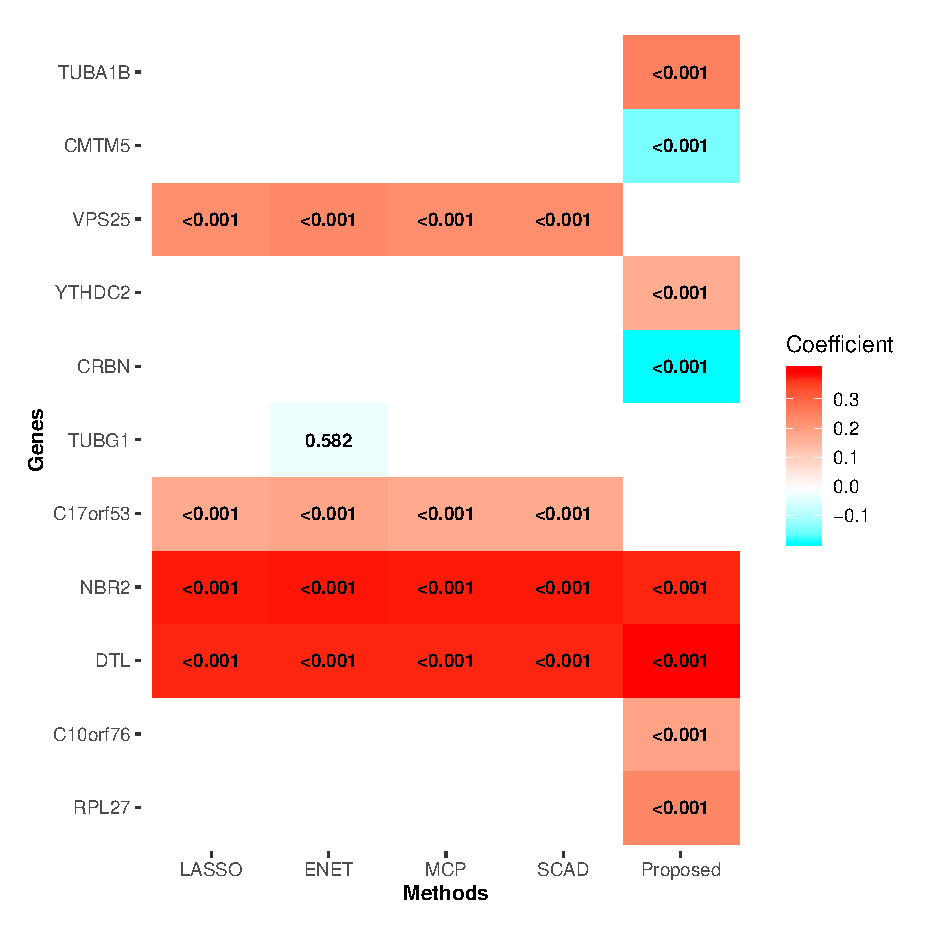
\includegraphics[width=0.48\textwidth]{heatmap.eps}
\caption{A heatmap of OLS coefficient estimates for the selected predictors with p-values.\label{Fig:heatmap}}
\end{figure}

\begin{table}[ht]
	\centering
	\begin{tabular}{rrrrr}
		\hline
		& NSP & MSE\_Pred & BIC & EBIC \\ 
		\hline
		Proposed & 8.00 & 0.60 & 985.93 & 1120.87 \\ 
		SCAD & 4.00 & 0.68 & 1104.69 & 1176.42 \\ 
		MCP & 4.00 & 0.68 & 1104.69 & 1176.42 \\ 
		ENET & 5.00 & 0.68 & 1110.65 & 1198.68 \\ 
		LASSO & 4.00 & 0.68 & 1104.69 & 1176.42 \\ 
		\hline
	\end{tabular}
\end{table}

\begin{figure}
	\centering
	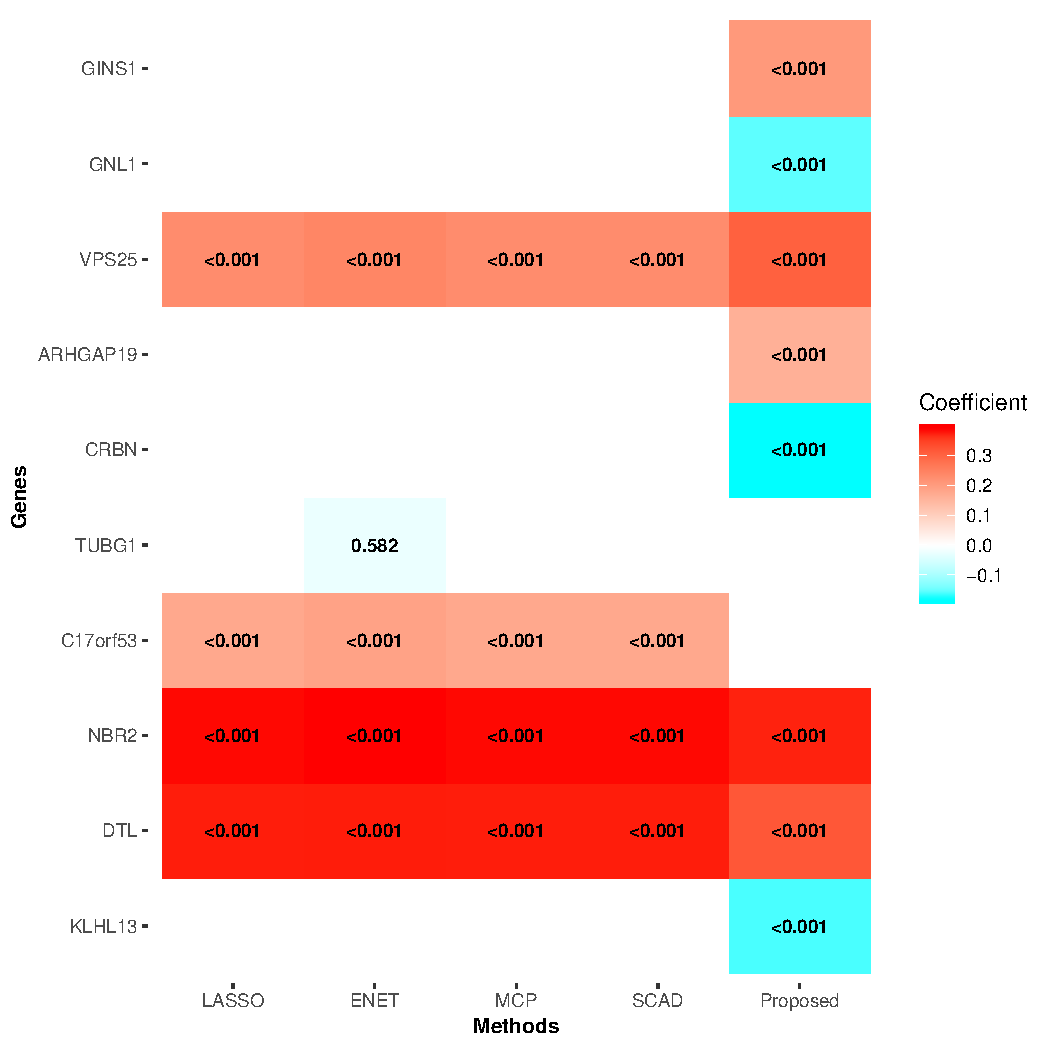
\includegraphics[width=0.48\textwidth]{heatmap1.pdf}
	\caption{A heatmap of OLS coefficient estimates for the selected predictors with p-values without screening.\label{Fig:heatmap1}}
\end{figure}

\section{Discussion}
The proposed hybrid search approach is computationally beneficial and practically effective compared with traditional stochastic search algorithms that are commonly used in Bayesian variable selection. Although the idea of searching over the neighborhood is somewhat similar to that of the MCMC model composition (MC$^3$) algorithm \citep{madigan1995bayesian} and the shotgun stochastic search (SSS) algorithm \citep{hans2007shotgun}, our search strategy is completely different from the existing methods. While MC$^3$ and SSS perform a stochastic search over the model space of all possible candidates, we implement a hybrid search over the sub-model space of size $k$. In addition, evaluating multiple candidates for the next move can be done simultaneously in a single computation in the proposed method.

In addition, as mentioned in Section \ref{sec:4}, parallel computing, which executes many calculations simultaneously using multiple nodes or multiple processors, can be employed in the proposed framework. Our hybrid search algorithm can be also extended to multivariate regression and binary regression in a Bayesian framework. Such works are in progress by the authors.


\appendix
\section{Calculation of Equation (3)}\label{app:1}
For any $i \notin \hat{\bg}$, from Eq. \eqref{eq:2}, we have
\begin{eqnarray}
\nonumber m(\uy|\hat{\bg}\cup\{i\})&\propto& |\uX_{\hat{\bg}\cup\{i\} }^{\T}\uX_{\hat{\bg}\cup\{i\} }+\tau^{-1}\uI_{k+1} |^{-1/2} \\
 \label{fact:0}&&\times \left(\uy^{\T}\uH_{\hat{\bg}\cup\{i\}}\uy+b_{\sigma}\right)^{-\frac{a_{\sigma}+n}{2} }.
\end{eqnarray}
It follows from the Sherman-Morrison formula that
\begin{eqnarray}\label{fact:1}
\uH_{\hat{\bg}\cup\{i\} }= \uH_{\hat{\bg}}-\frac{\uH_{\hat{\bg}}\ux_i \ux_i
	^{\T}\uH_{\hat{\bg}} } {\tau^{-1}+\ux_i^{\T}\uH_{\hat{\bg}}\ux_i}.
\end{eqnarray}
Using the Sylvester's determinant identity and the Sherman-Morrison formula, we obtain 
\begin{eqnarray}
	\nonumber &&|\uX_{\hat{\bg}\cup\{i\} }^{\T}\uX_{\hat{\bg}\cup\{i\} }+\tau^{-1}\uI_{k+1}   | \\
	\nonumber &&= \tau^{-(k+1)}|\tau \uX_{\hat{\bg}\cup\{i\} }\uX_{\hat{\bg}\cup\{i\} }^{\T}+\uI_n |\nonumber\\
	\nonumber &&= \tau^{-(k+1)}|\tau \uX_{\hat{\bg}}\uX_{\hat{\bg}}^{\T}+\uI_n+\tau \ux_i \ux_i^{\T} |\nonumber\\
	\nonumber &&=  \tau^{-(k+1)} |\tau \uX_{\hat{\bg}}\uX_{\hat{\bg}}^{\T}+\uI_n| \{1+ \tau \ux_i^{\T}
	(\tau \uX_{\hat{\bg}}\uX_{\hat{\bg}}^{\T}+\uI_n)^{-1}\ux_i\}\nonumber\\
	\label{fact:2} &&=| \uX_{\hat{\bg}}^{\T}\uX_{\hat{\bg}}+\tau^{-1}\uI_{k}| (\tau^{-1}+\ux_i^{\T}\uH_{\hat{\bg}} \ux_i).
\end{eqnarray}
Applying \eqref{fact:1} and \eqref{fact:2} to \eqref{fact:0}, we thus have
\begin{eqnarray*}
 m(\uy|\hat{\bg}\cup\{i\}) &\propto& \left\{\uy^{\T}\uH_{\hat{\bg}}\uy-\frac{(
 	\ux_i^{\T}\uH_{\hat{\bg}}\uy)^2}{\tau^{-1}+\ux_i^{\T}\uH_{\hat{\bg}} \ux_i }+b_{\sigma}\right\}^
 {-\frac{a_{\sigma}+n}{2}}\\
 &&\times (\tau^{-1}+\ux_i^{\T}\uH_{\hat{\bg}} \ux_i)^{-1/2}
\end{eqnarray*}
for any $i \notin \hat{\bg}$. 

\section{Calculation of Equation (4)}\label{app:2}
For any $j \in \tilde{\bg}$, Eq. \eqref{eq:2} leads to
\begin{eqnarray}
\nonumber m(\uy|\tilde{\bg}\setminus\{j\})&\propto& |\uX_{\tilde{\bg}\setminus\{j\} }^{\T}\uX_{\tilde{\bg}\setminus\{j\}}+\tau^{-1}\uI_{k} |^{-1/2} \\
 \label{fact:0-1}&&\times  \left(\uy^{\T}\uH_{\tilde{\bg}\setminus\{j\}}\uy+b_{\sigma}\right)^{-\frac{a_{\sigma}+n}{2} }.
\end{eqnarray}
From the Sherman-Morrison formula, we have
\begin{eqnarray}\label{fact:1-1}
\uH_{\tilde{\bg}\setminus\{j\} }= \uH_{\tilde{\bg}}+\frac{\uH_{\tilde{\bg}}\ux_j \ux_j
	^{\T}\uH_{\tilde{\bg}} } {\tau^{-1}-\ux_j^{\T}\uH_{\tilde{\bg}}\ux_j}.
\end{eqnarray}
From the Sylvester's determinant identity and the Sherman-Morrison formula, we obtain 
\begin{eqnarray}
	\nonumber &&|\uX_{\tilde{\bg}\setminus\{j\}}^{\T}\uX_{\tilde{\bg}\setminus\{j\} }+\tau^{-1}\uI_{k}   | \\
	&&= \tau^{-k}|\tau \uX_{\tilde{\bg}\setminus\{j\} }\uX_{\tilde{\bg}\setminus\{j\} }^{\T}+\uI_n |\nonumber\\
	&&= \tau^{-k}|\tau \uX_{\tilde{\bg}}\uX_{\tilde{\bg}}^{\T}+\uI_n-\tau \ux_j \ux_j^{\T} |\nonumber\\
	&&=  \tau^{-k} |\tau \uX_{\tilde{\bg}}\uX_{\tilde{\bg}}^{\T}+\uI_n| \{1- \tau \ux_j^{\T}
	(\tau \uX_{\tilde{\bg}}\uX_{\tilde{\bg}}^{\T}+\uI_n)^{-1}\ux_j\}\nonumber\\
	\label{fact:2-1} &&=\tau^2 | \uX_{\tilde{\bg}}^{\T}\uX_{\tilde{\bg}}+\tau^{-1}\uI_{k+1}| (\tau^{-1}-\ux_j^{\T}\uH_{\tilde{\bg}} \ux_j).
\end{eqnarray}
Hence, applying \eqref{fact:1-1} and \eqref{fact:2-1} to \eqref{fact:0-1}, we have
\begin{eqnarray*}
&&m(\uy|\tilde{\bg}\setminus \{j\})  \propto \left\{\uy^{\T}\uH_{\tilde{\bg}}\uy+\frac{(
 	\ux_j^{\T}\uH_{\tilde{\bg}}\uy)^2}{\tau^{-1}-\ux_j^{\T}\uH_{\tilde{\bg}} \ux_j }+b_{\sigma}\right\}^
 {-\frac{a_{\sigma}+n}{2}}\\
 &&\times (\tau^{-1}-\ux_j^{\T}\uH_{\tilde{\bg}} \ux_j)^{-1/2}
\end{eqnarray*}
for any $j \in \tilde{\bg}$.


\bibliographystyle{spbasic} 
\bibliography{Ref_Bayes_Subset}


\end{document}
% end of file template.tex

